\section{Online Insertion}
In the preceeding section we showed that it is possible to break a large 
number of path symmetries by decomposing a 4-connected grid map into 
a set of empty rectangular rooms and pruning all nodes from the interior of
each room.
However, it is often the case that a pruned node might be required at a later
point as a start or goal location for an agent.
To solve this problem we propose to insert these  nodes
back into the graph for the duration of the search using the following procedure (highlighted in Figure \ref{fig:insertion}):
\begin{enumerate}
\item{If the start and goal are in the same room no insertion is required.
 Since it is guaranteed that there are no obstacles between the two locations, an optimal 
 path is trivially available. This case will be ignored in the rest of our discussion.}
% take the Manhattan distance between them as the length of the optimal path. }
\item{If the start and goal are not in the same room, connect each of them
to the closest neighbours on each side of the perimeter of the empty room.}
\end{enumerate}
We claim that this procedure allows to retain optimal paths from the start (or goal) location
to all nodes of the perimeter of its room.

\begin{figure}[t]
	\vspace{-4pt}
       \begin{center}
           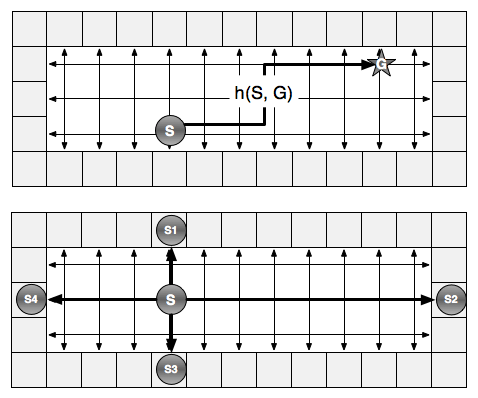
\includegraphics[scale=0.50, trim = 10mm 10mm 10mm 0mm]{diagrams/roomtraversal.png}
       \end{center}
	\vspace{-3pt}
       \caption{(Top) When $S$ and $G$ are in the empty room no insertion is necessary.
				(Bottom) $S$ is a previously pruned interior node.
				We insert $S$ into the graph and connect it to neighbours on each side of the empty room.}
	%\vspace{-15pt}
	\label{fig:insertion}
\end{figure}

\begin{lemma}
\label{thm-insertion}
Let $R$ be an empty rectangular room.
For any nodes $m, n$, with $m$ a re-inserted interior node and $n$ a node on the perimeter,
it is always possible to find an optimal length path which mentions no interior nodes except for $m$.
\end{lemma}
\begin{proof}
We insert $m$ into the graph and connect it to 
$s'_{1}, s'_{2}, s'_{3}, s'_{4}$, the closest neighbours on 
each side of the perimeter.
The weight of each edge incident with $m$ is equal to the Manhattan distance between
$m$ and each $s'_{i}$.
To find an optimal path to $n$ we travel from $m$ to the node $s'_{i}$ which is 
on the same side as $n$ on the perimeter.
From there we travel along the perimeter of $R$ until we reach $n$.
%\par
%Next, suppose $s, g \in N$. 
%In this case we do not insert anything; the length of the optimal path is equal
%to the Manhattan distance between $s$ and $g$.
\end{proof}

Once the search has finished we remove the start and goal from the graph.
The time required in each case (insertion and deletion) is constant.

\section{Optimality}
We claim that procedure outlined earlier is sufficient to 
guarantee that running A* on our pruned maps will always return an optimal solution if one exists.

\begin{theorem}
For every optimal length path $\pi^*(s, g)$ in a 4-connected grid map there exists
an equivalent length path in the pruned version of the grid map.
\end{theorem}
\begin{proof}
Follows from Lemma \ref{thm-roomtraversal} and Lemma \ref{thm-insertion}.
For every optimal length segment of $\pi^{*}(s, g)$ which traverses
through an empty room there is an equivalent segment which mentions only nodes
on the perimeter of each room (and possibly one macro-step).
%Thus the length of $\pi'(s, g)$ is equal to the length of $\pi'(s,g)$.
\end{proof}

If desired, optimal solutions pruned by our symmetry reduction can easily be reconstructed
from our optimal solutions.
Consider a path fragment between $m$ and $n$, two nodes on the perimeter of an empty room.
Assume, without any generality loss, that the path fragment contains $r$ moves to the right and $u$ moves upwards.
All optimal path fragments between $m$ and $n$ can be obtained by interleaving $r$ moves to the right
and $u$ moves upwards in any order.

\begin{figure}[t]
%	\vspace{-4pt}
\centering
	    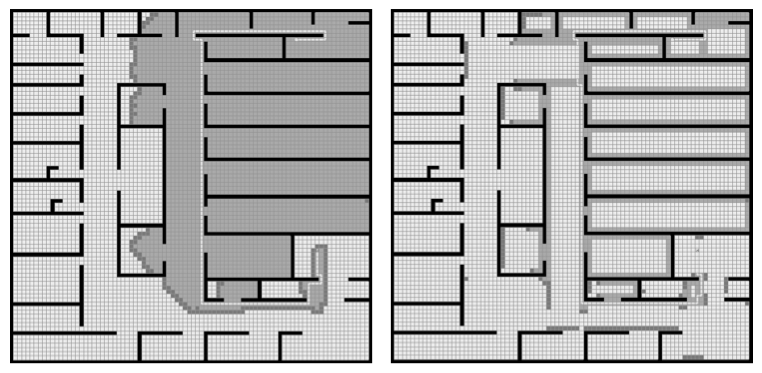
\includegraphics[width=0.95\columnwidth, trim = 10mm 10mm 10mm 0mm]{diagrams/oha_contrast.png}
		\caption{Left: A* solving a problem on an unmodified ($86\times88$) grid map. 
		Expanded nodes are marked light grey while nodes at the frontier are dark grey.
		Right: A* solving the same problem using our modified grid map. 
		The algorithm only considers nodes along the perimeter of the identified rooms.}
	\label{fig-contrast}
\end{figure}

In Figure \ref{fig-contrast} we highlight the effectiveness of our symmetry breaking technique using
a map that has characteristics typical of what one might expect in a modern role-playing game \footnote{
Infact, most video game maps tend to be somewhat bigger than our example but for demonstration 
purposes it is quite sufficient.}
; there are many rooms and corridors and many entrances connecting them.
Using A* we solve a typical problem on the original grid map and in the process expand almost half the nodes
in the state space.
We then decompose the map to eliminate symmetries and re-run A*.
This time A* expands less than 15\% of all nodes (more than a three-fold improvement) and returns the 
optimal solution 4 times faster.
